\documentclass[11pt,a4paper]{article}

% Packages
\usepackage[utf8]{inputenc}
\usepackage[T1]{fontenc}
\usepackage{geometry}
\usepackage{graphicx}
\usepackage{booktabs}
\usepackage{amsmath}
\usepackage{amssymb}
\usepackage{hyperref}
\usepackage{caption}
\usepackage{subcaption}
\usepackage{float}
\usepackage{enumitem}
\usepackage{xcolor}
\usepackage{fancyhdr}
\usepackage{titlesec}
\usepackage{multirow}
\usepackage{array}
\usepackage{longtable}
\usepackage{tabularx}

% Page geometry
\geometry{margin=2.5cm}

% Header/Footer
\pagestyle{fancy}
\fancyhf{}
\rhead{Machine Learning - Homework 2}
\lhead{Davide De Blasio - 2082600}
\rfoot{\thepage}

% Title format
\titleformat{\section}{\Large\bfseries}{\thesection}{1em}{}
\titleformat{\subsection}{\large\bfseries}{\thesubsection}{1em}{}

% Hyperlink setup
\hypersetup{
    colorlinks=true,
    linkcolor=blue,
    filecolor=magenta,
    urlcolor=cyan,
    citecolor=blue
}

\begin{document}

% Title Page
\begin{titlepage}
    \centering
    \vspace*{2cm}
    
    {\Huge\bfseries Machine Learning\\[0.5cm]Homework 2 Report\par}
    
    \vspace{2cm}
    
    {\Large Comprehensive Analysis of Dimensionality Reduction\\Techniques Across Three Machine Learning Tasks\par}
    
    \vspace{3cm}
    
    {\large\textbf{Author:} Davide De Blasio\\[0.3cm]
    \textbf{Student ID:} 2082600\\[0.3cm]
    \textbf{Date:} January 2026\par}
    
    \vfill
    
    {\large
    \textbf{Tasks Completed:}\\[0.5cm]
    \begin{tabular}{ll}
        1. & Waste Classification with Convolutional Neural Networks\\
        2. & Customer Segmentation with K-Means Clustering\\
        3. & Life Expectancy Prediction with Feedforward Neural Networks\\
    \end{tabular}
    \par}
    
    \vspace{1cm}
    
\end{titlepage}

\tableofcontents
\newpage

%==============================================================================
\section{Introduction and Motivation}
%==============================================================================

This report presents a comprehensive analysis of three machine learning tasks, each addressing a distinct learning paradigm: supervised classification, unsupervised clustering, and regression. The unifying theme across all tasks is the systematic comparison of model performance when trained on:

\begin{enumerate}
    \item \textbf{Original features} -- full-dimensional input data
    \item \textbf{PCA-reduced features} -- linear dimensionality reduction
    \item \textbf{Autoencoder-reduced features} -- non-linear dimensionality reduction
\end{enumerate}

\subsection{Motivation}

Dimensionality reduction is crucial in modern machine learning for several reasons:

\begin{itemize}
    \item \textbf{Computational Efficiency:} High-dimensional data increases training time and memory requirements
    \item \textbf{Curse of Dimensionality:} As dimensions increase, data becomes increasingly sparse, making pattern recognition more difficult
    \item \textbf{Noise Reduction:} Irrelevant features can introduce noise that degrades model performance
    \item \textbf{Interpretability:} Lower-dimensional representations can reveal latent structure in the data
\end{itemize}

By comparing linear (PCA) and non-linear (Autoencoder) reduction techniques across classification, clustering, and regression tasks, we gain insight into when each approach is most effective and the trade-offs involved.

\subsection{Task Overview}

\begin{table}[H]
\centering
\caption{Summary of Machine Learning Tasks}
\begin{tabular}{@{}llll@{}}
\toprule
\textbf{Task} & \textbf{Type} & \textbf{Model} & \textbf{Dataset} \\
\midrule
Waste Classification & Multi-class Classification & CNN & \href{https://www.kaggle.com/datasets/joebeachcapital/realwaste}{RealWaste} \\
Customer Segmentation & Unsupervised Clustering & K-Means & \href{https://www.kaggle.com/datasets/henrysue/online-shoppers-intention}{Online Shopper's Intention} \\
Life Expectancy & Regression & FNN & \href{https://www.kaggle.com/datasets/kumarajarshi/life-expectancy-who}{Life Expectancy WHO} \\
\bottomrule
\end{tabular}
\end{table}

%==============================================================================
\section{Dataset Description}
%==============================================================================

\subsection{Task 1: Waste Classification (RealWaste Dataset)}

The RealWaste dataset from Kaggle contains images of waste materials for automated waste sorting applications.

\begin{table}[H]
\centering
\caption{RealWaste Dataset Characteristics}
\begin{tabular}{@{}ll@{}}
\toprule
\textbf{Property} & \textbf{Value} \\
\midrule
Source & Kaggle (RealWaste) \\
Task Type & Multi-class Image Classification \\
Number of Classes & 9 \\
Image Format & RGB Images \\
Split Ratio & 70\% Train / 15\% Validation / 15\% Test \\
\bottomrule
\end{tabular}
\end{table}

\textbf{Classes:} Cardboard, Food Organics, Glass, Metal, Miscellaneous Trash, Paper, Plastic, Textile Trash, Vegetation

\begin{figure}[H]
    \centering
    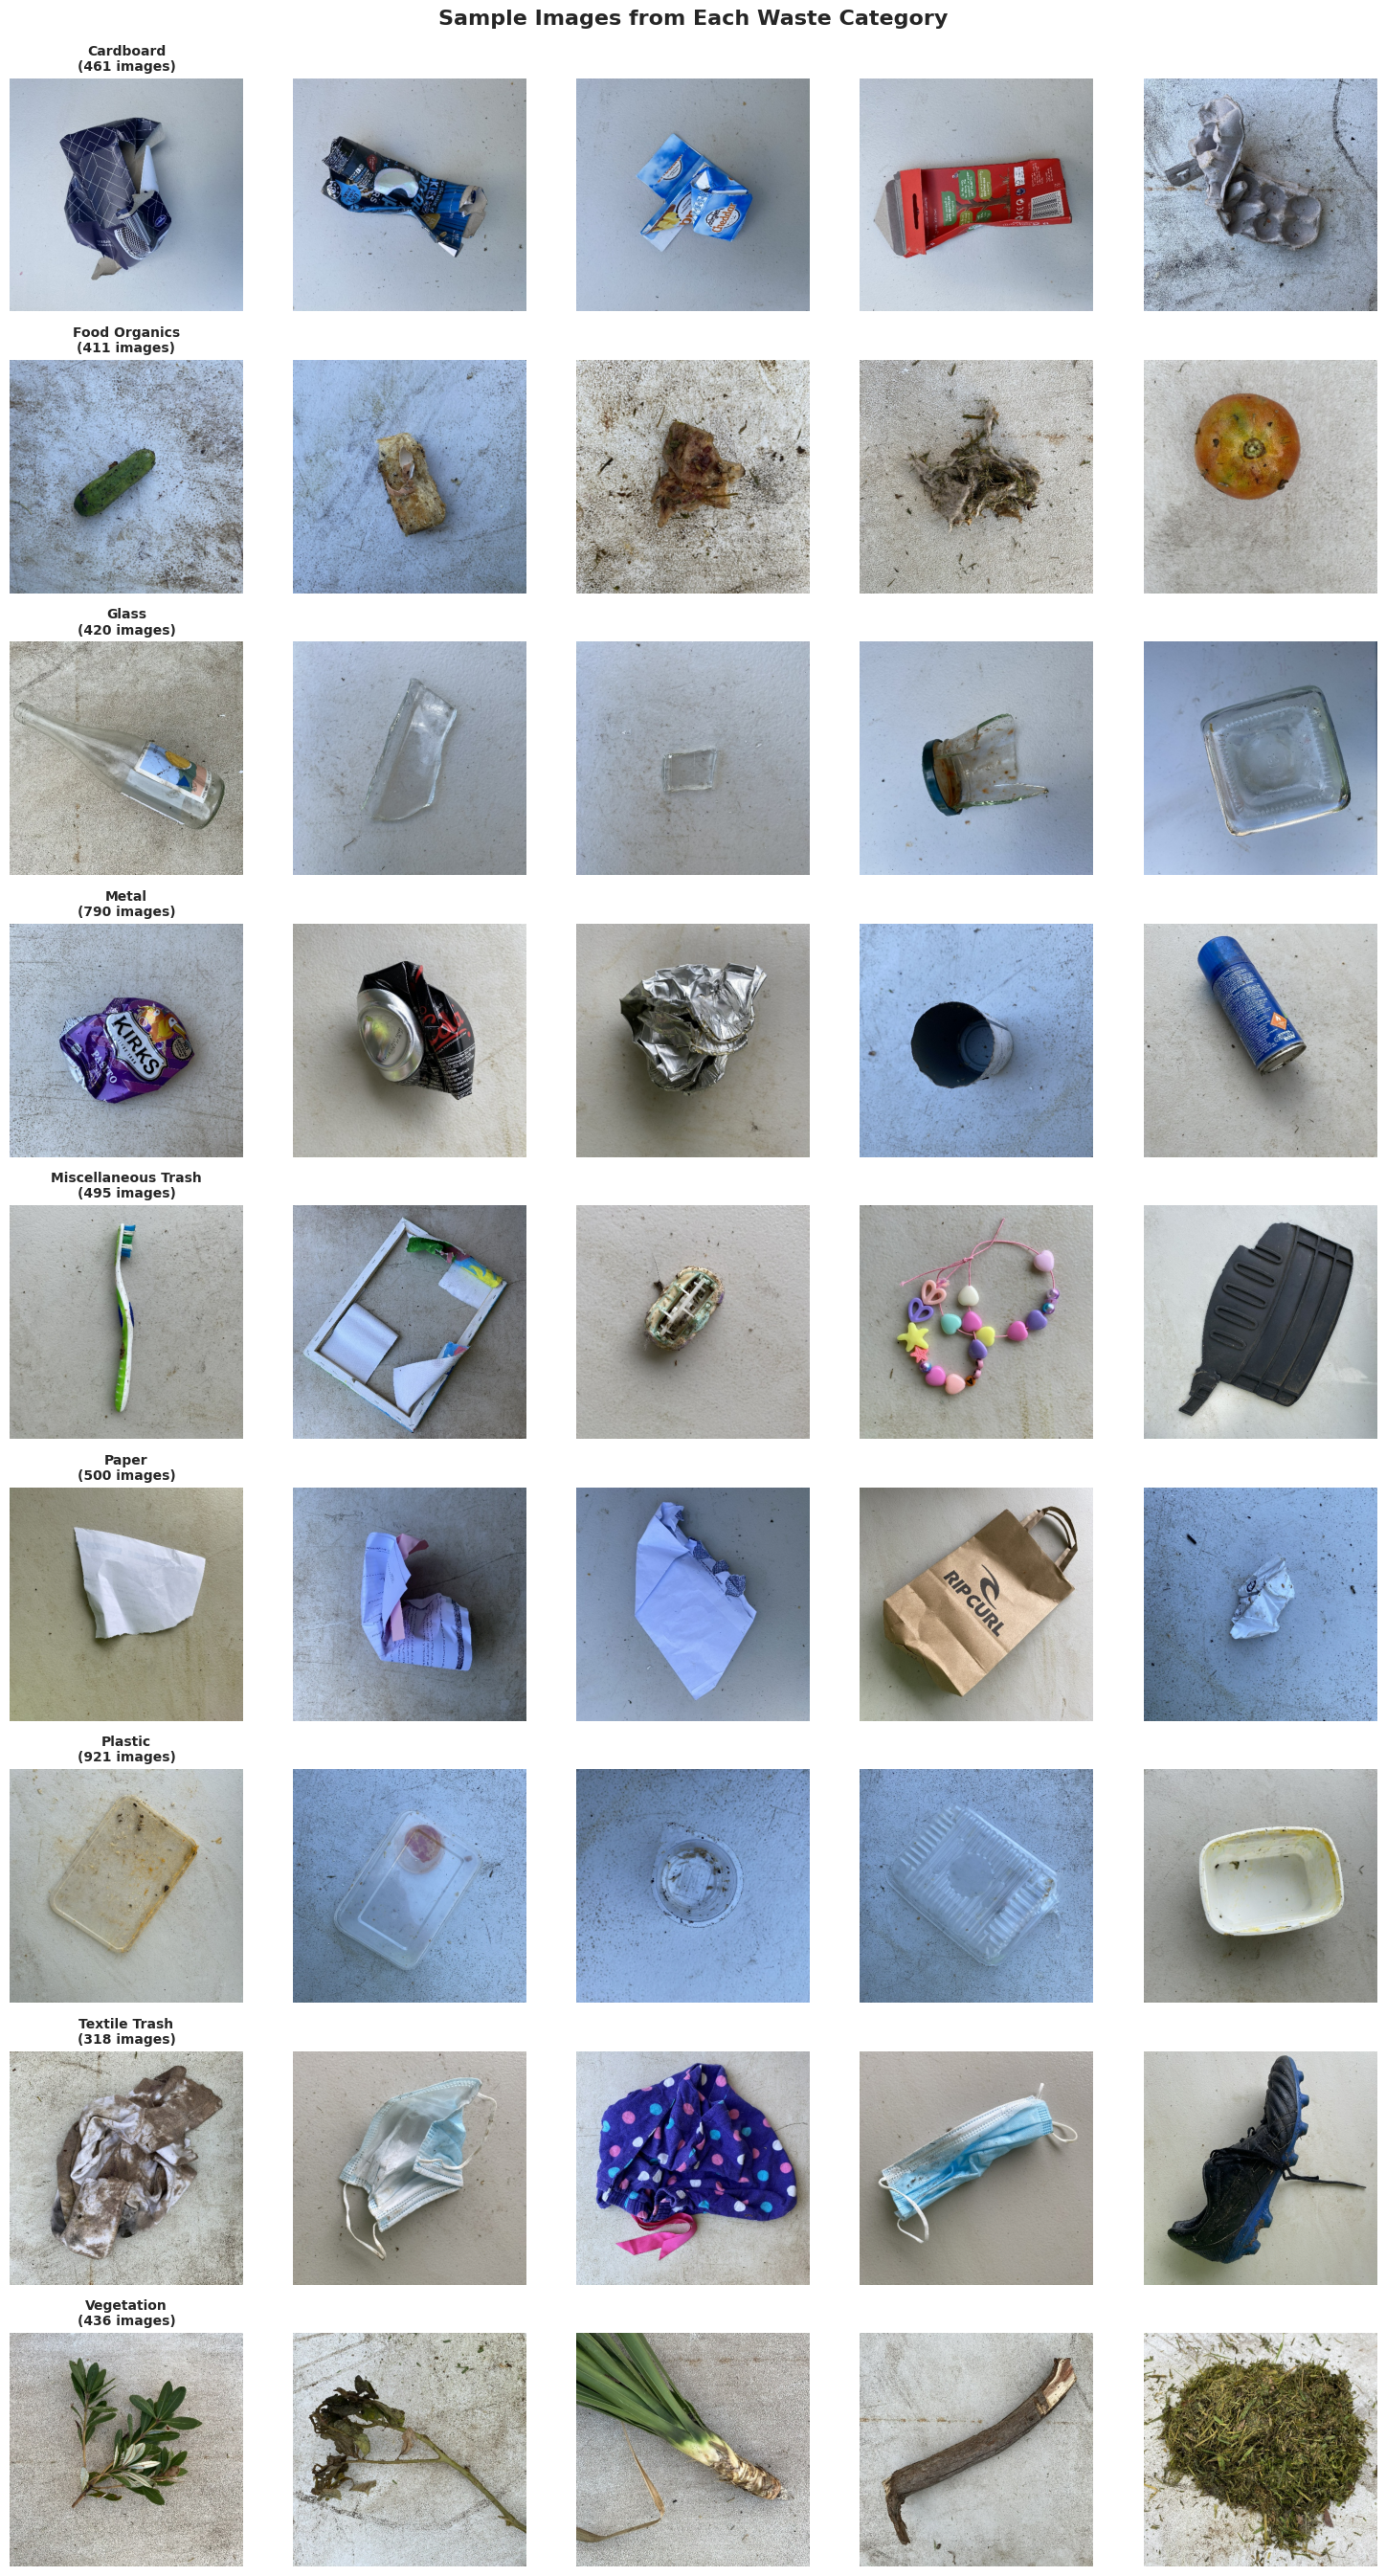
\includegraphics[width=0.6\textwidth]{waste_list.png}
    \caption{Distribution of waste categories in the RealWaste dataset}
    \label{fig:waste_class_distribution}
\end{figure}

\subsection{Task 2: Customer Segmentation (Online Shopper's Intention Dataset)}

This dataset captures browsing behavior of online shoppers for customer segmentation analysis.

\begin{table}[H]
\centering
\caption{Online Shopper's Intention Dataset Characteristics}
\begin{tabular}{@{}ll@{}}
\toprule
\textbf{Property} & \textbf{Value} \\
\midrule
Source & Kaggle (Online Shopper's Intention) \\
Samples & 12,330 sessions \\
Features & 17 (after preprocessing) \\
Missing Values & Minimal \\
Split Ratio & 60\% Train / 20\% Validation / 20\% Test \\
\bottomrule
\end{tabular}
\end{table}

\textbf{Key Features:} Administrative pages, Informational pages, Product-related pages, Bounce rates, Exit rates, Page values, Special day indicators, Month, Operating system, Browser, Region, Traffic type, Visitor type, Weekend indicator.

\begin{figure}[H]
    \centering
    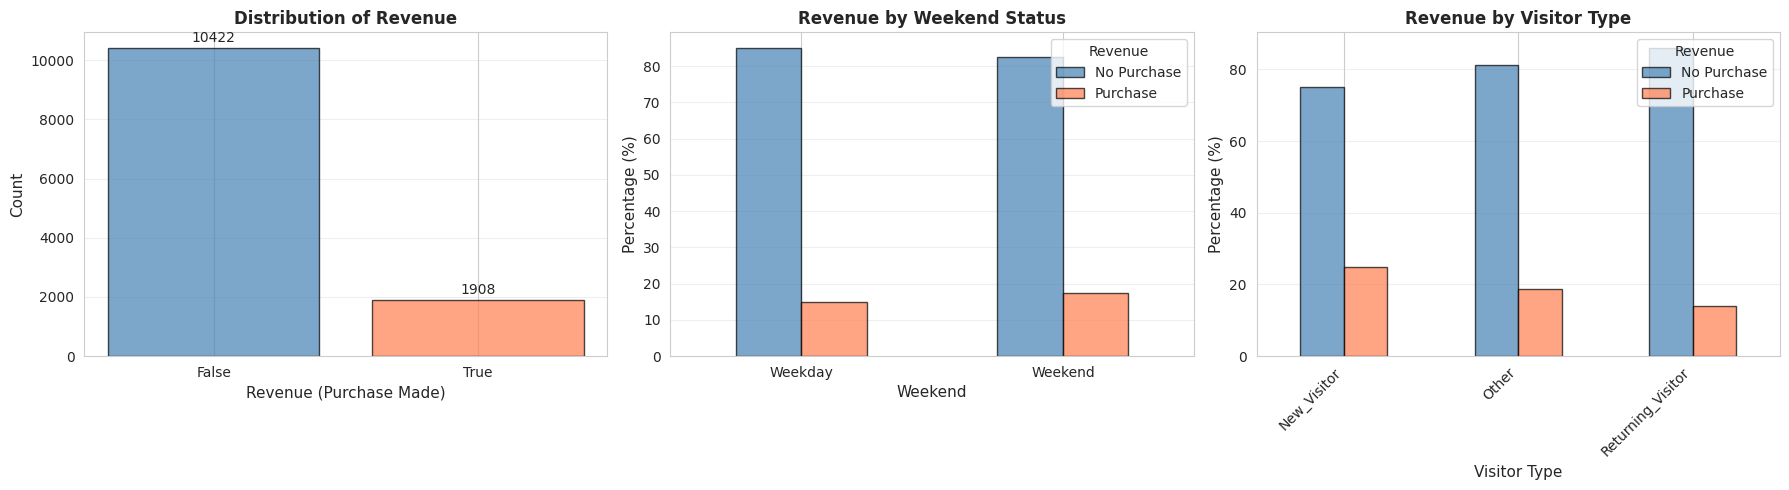
\includegraphics[width=1\textwidth]{revenue.png}
    \caption{Distribution of Revenue and analysis by Visitor Type}
    \label{fig:customer_distribution}
\end{figure}

\subsection{Task 3: Life Expectancy Prediction (WHO Dataset)}

The Life Expectancy WHO dataset contains health, economic, and demographic indicators for countries worldwide.

\begin{table}[H]
\centering
\caption{Life Expectancy WHO Dataset Characteristics}
\begin{tabular}{@{}ll@{}}
\toprule
\textbf{Property} & \textbf{Value} \\
\midrule
Source & Kaggle (Life Expectancy WHO) \\
Samples & 2,938 records \\
Features & 20 original predictive features (208 after one-hot encoding) \\
Target Variable & Life Expectancy (years) \\
Missing Values & Present (handled via KNN Imputation) \\
Split Ratio & 60\% Train / 20\% Validation / 20\% Test \\
\bottomrule
\end{tabular}
\end{table}

\textbf{Key Features:} Adult Mortality, Infant Deaths, Alcohol consumption, Health Expenditure, Hepatitis B immunization, Measles cases, BMI, Under-five deaths, Polio immunization, Diphtheria immunization, HIV/AIDS prevalence, GDP, Population, Schooling, Income Composition.

\begin{figure}[H]
    \centering
    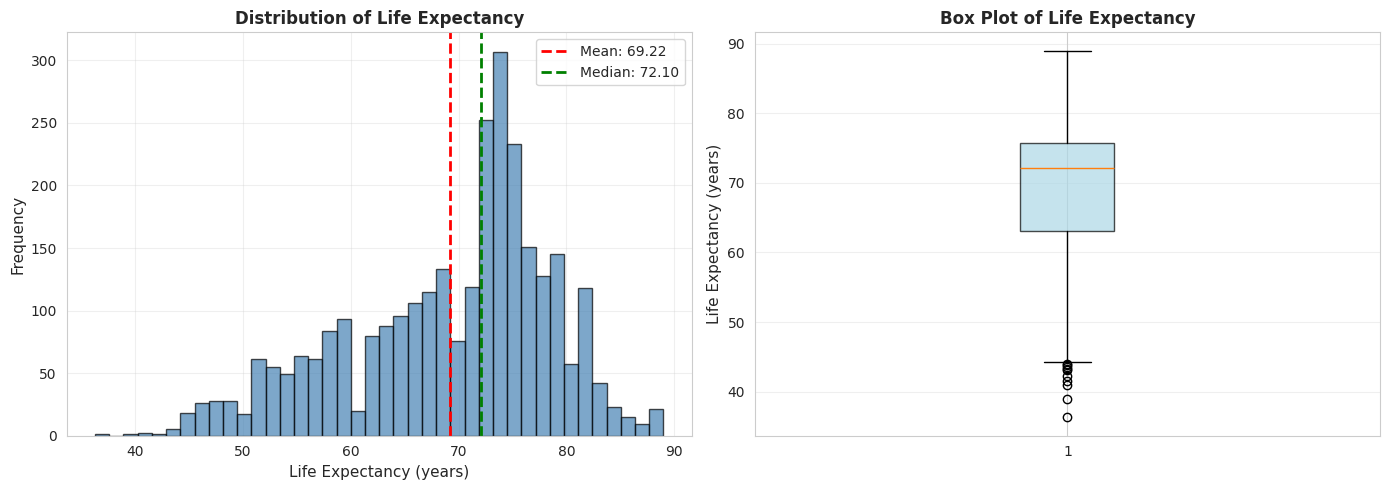
\includegraphics[width=1\textwidth]{life_expectacy.png}
    \caption{Distribution of the target variable (Life Expectancy)}
    \label{fig:life_expectancy_distribution}
\end{figure}

%==============================================================================
\section{Methodology and Models}
%==============================================================================

\subsection{Common Preprocessing Pipeline}

All three tasks follow a consistent preprocessing methodology:

\begin{enumerate}
    \item \textbf{Data Splitting:} Train/Validation/Test split performed \textit{before} any scaling to prevent data leakage
    \item \textbf{Feature Scaling:} StandardScaler (or MinMaxScaler for regression) fitted only on training data
    \item \textbf{Missing Value Handling:} KNN Imputation (for Life Expectancy dataset)
    \item \textbf{Categorical Encoding:} Label encoding for categorical variables
    \item \textbf{Reproducibility:} Random seeds set to 42 for all experiments
\end{enumerate}

\subsubsection{Task 1: Waste Classification Preprocessing}

\textbf{Image Preprocessing:}
\begin{itemize}
    \item Image resizing to $128 \times 128$ pixels (IMG\_SIZE = 128)
    \item Conversion to RGB format
    \item Normalization using ImageNet statistics: mean = [0.485, 0.456, 0.406], std = [0.229, 0.224, 0.225]
\end{itemize}

\textbf{Data Augmentation (Training Only):}
\begin{itemize}
    \item \textbf{RandomHorizontalFlip:} $p = 0.5$ - randomly flips images horizontally to increase orientation invariance
    \item \textbf{RandomRotation:} $\pm 10^\circ$ - small rotations to simulate real-world variations in waste positioning
\end{itemize}

\textbf{Feature Extraction:}
\begin{itemize}
    \item Pre-trained ResNet18 (frozen weights) used as feature extractor
    \item Output: 512-dimensional feature vectors per image
    \item StandardScaler applied to extracted features (fitted on training set only)
\end{itemize}

\subsubsection{Task 2: Customer Clustering Preprocessing}

\begin{itemize}
    \item \textbf{Missing Values:} Filled with 0 (minimal missing data)
    \item \textbf{Categorical Encoding:} LabelEncoder applied to Month, VisitorType, Weekend, and Revenue columns
    \item \textbf{Feature Scaling:} StandardScaler fitted on training data, applied to all splits
    \item \textbf{Final Features:} 17 numerical features after preprocessing
\end{itemize}

\subsubsection{Task 3: Life Expectancy Preprocessing}

\begin{itemize}
    \item \textbf{Missing Values:} KNN Imputation with $k = 5$ neighbors
    \item \textbf{Outlier Handling:} IQR-based capping on numerical features
    \item \textbf{Categorical Encoding:} One-hot encoding for Country and Status (with drop\_first=True)
    \item \textbf{Feature Selection:} Removal of highly correlated features (under-five deaths, percentage expenditure, thinness 5-9 years, Schooling)
    \item \textbf{Feature Scaling:} MinMaxScaler fitted on training data
    \item \textbf{Final Features:} 208 features after one-hot encoding
\end{itemize}

\subsection{Dimensionality Reduction Techniques}

\subsubsection{PCA (Principal Component Analysis)}

PCA performs linear dimensionality reduction by projecting data onto orthogonal principal components that maximize variance.

\begin{equation}
    \mathbf{X}_{reduced} = \mathbf{X} \cdot \mathbf{W}_k
\end{equation}

where $\mathbf{W}_k$ contains the top $k$ eigenvectors of the covariance matrix.

\textbf{Target Dimensions:}
\begin{itemize}
    \item Customer Clustering: 13 components (94\% variance retained)
    \item Life Expectancy: 145 components (90\% of variance retained)
    \item Waste Classification: 256 components (from 512 ResNet18 features)
\end{itemize}

\begin{figure}[H]
    \centering

    \begin{subfigure}{0.8\textwidth}
        \centering
        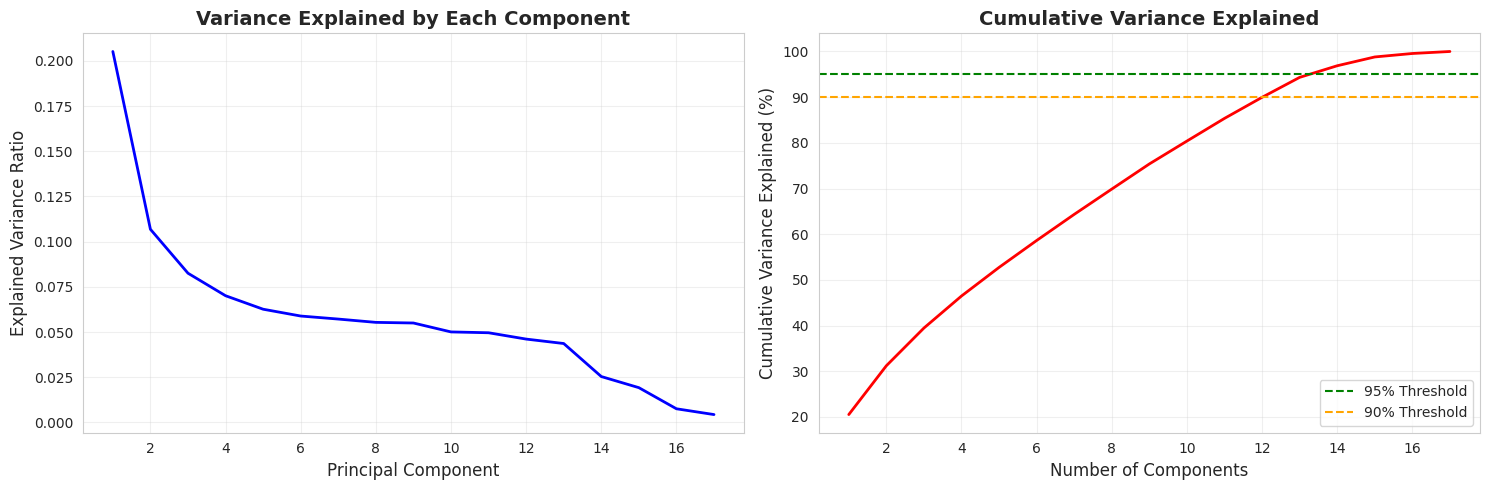
\includegraphics[width=\linewidth]{pca_customer.png}
        \caption{Customer Clustering}
    \end{subfigure}

    \vspace{0.5cm}

    \begin{subfigure}{0.8\textwidth}
        \centering
        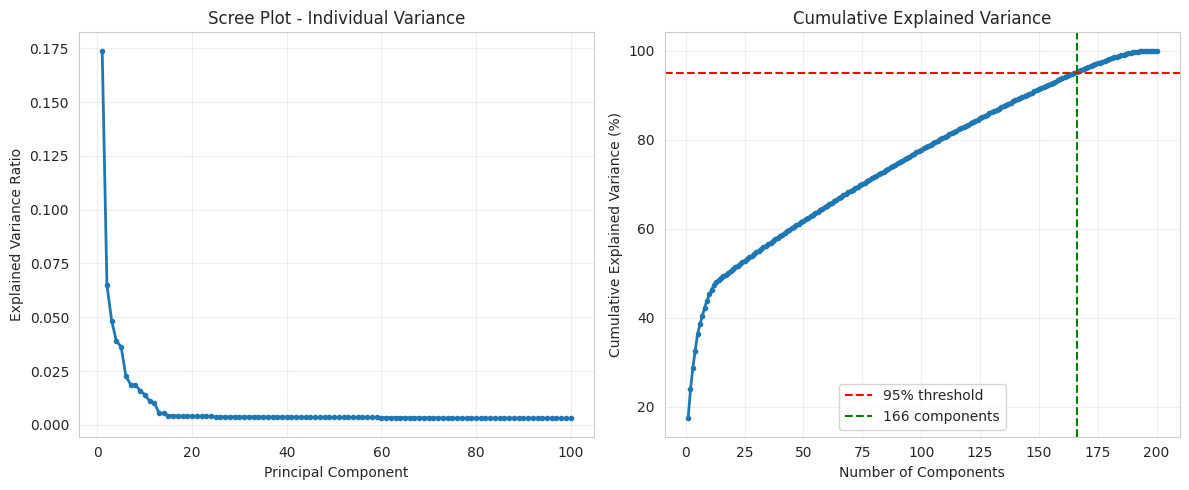
\includegraphics[width=\linewidth]{pca_life.png}
        \caption{Life Expectancy Regression}
    \end{subfigure}

    \vspace{0.5cm}

    \begin{subfigure}{0.8\textwidth}
        \centering
        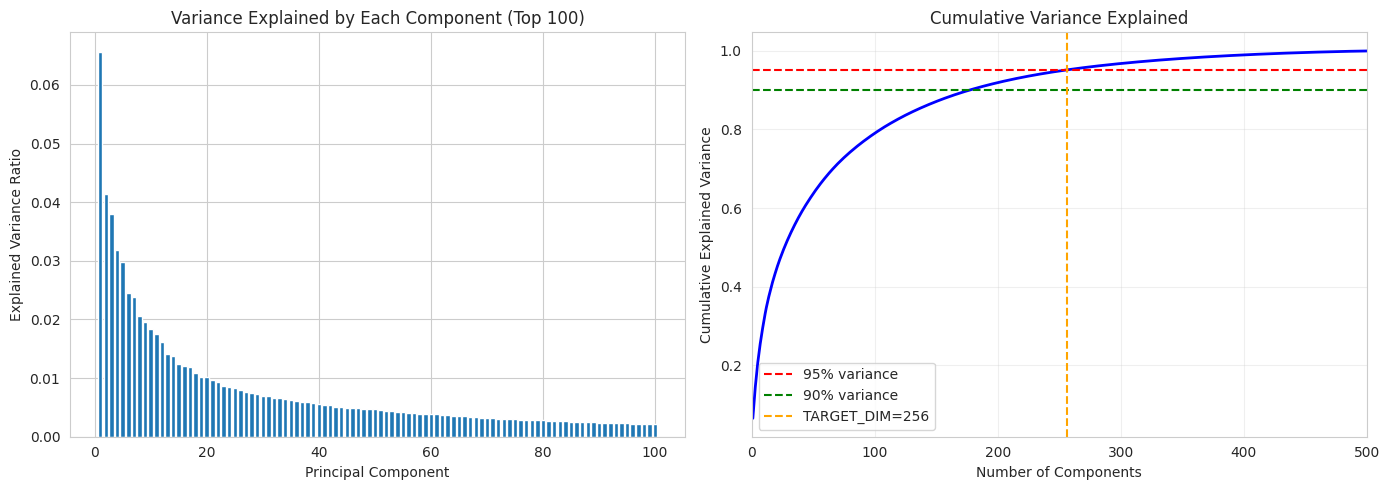
\includegraphics[width=\linewidth]{pca_waste.png}
        \caption{Waste Classification}
    \end{subfigure}

    \caption{Cumulative variance explained by principal components}
    \label{fig:pca_variance}
\end{figure}

\subsubsection{Autoencoder for Non-linear Reduction}

Autoencoders learn non-linear compressed representations through neural network encoding and decoding.

\textbf{Architecture (Customer/Life Expectancy):}
\begin{verbatim}
Encoder: Input -> 128 -> BatchNorm -> ReLU -> 64 -> BatchNorm -> ReLU -> Latent
Decoder: Latent -> 64 -> BatchNorm -> ReLU -> 128 -> BatchNorm -> ReLU -> Output
\end{verbatim}

\textbf{Architecture (Waste Classification):}
\begin{verbatim}
Encoder: 512 -> Dropout(0.4) -> Linear(512, 256) -> LayerNorm -> GELU
Decoder: Dropout(0.4) -> Linear(256, 512)
\end{verbatim}

\textbf{Training Parameters (Life Expectancy Regression):}
\begin{itemize}
    \item Optimizer: Adam (lr = 0.001, weight\_decay = 1e-4)
    \item Loss: Mean Squared Error (MSE)
    \item Early Stopping: Patience = 20 epochs
    \item Learning Rate Scheduler: ReduceLROnPlateau (factor = 0.5, patience = 10)
    \item Batch Size: 32
    \item Maximum Epochs: 150
\end{itemize}

\textbf{Training Parameters (Customer Clustering):}
\begin{itemize}
    \item Optimizer: Adam (lr = 0.001, weight\_decay = 1e-4)
    \item Loss: Mean Squared Error (MSE)
    \item Early Stopping: Patience = 20 epochs
    \item Learning Rate Scheduler: ReduceLROnPlateau (factor = 0.5, patience = 10)
    \item Batch Size: 32
    \item Maximum Epochs: 100
\end{itemize}

\textbf{Training Parameters (Waste Classification):}
\begin{itemize}
    \item Optimizer: AdamW (lr = 1e-3, weight\_decay = 1e-3)
    \item Loss: Smooth L1 Loss
    \item Early Stopping: Patience = 10 epochs
    \item Learning Rate Scheduler: ReduceLROnPlateau (factor = 0.5, patience = 5, min\_lr = 1e-6)
\end{itemize}

\begin{figure}[H]
    \centering

    \begin{subfigure}{0.50\textwidth}
        \centering
        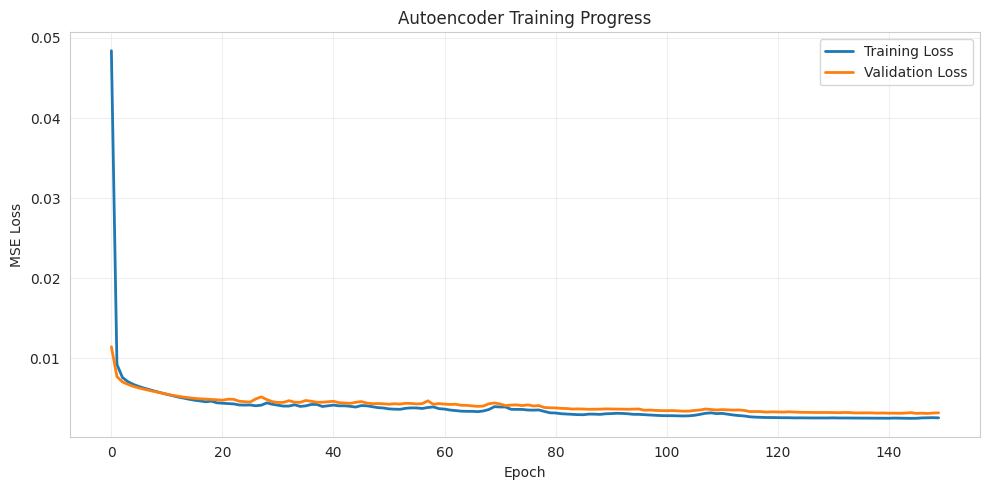
\includegraphics[width=\linewidth]{autoencoder_life.png}
        \caption{Life Expectancy Regression}
    \end{subfigure}
    \hfill
    \begin{subfigure}{0.43\textwidth}
        \centering
        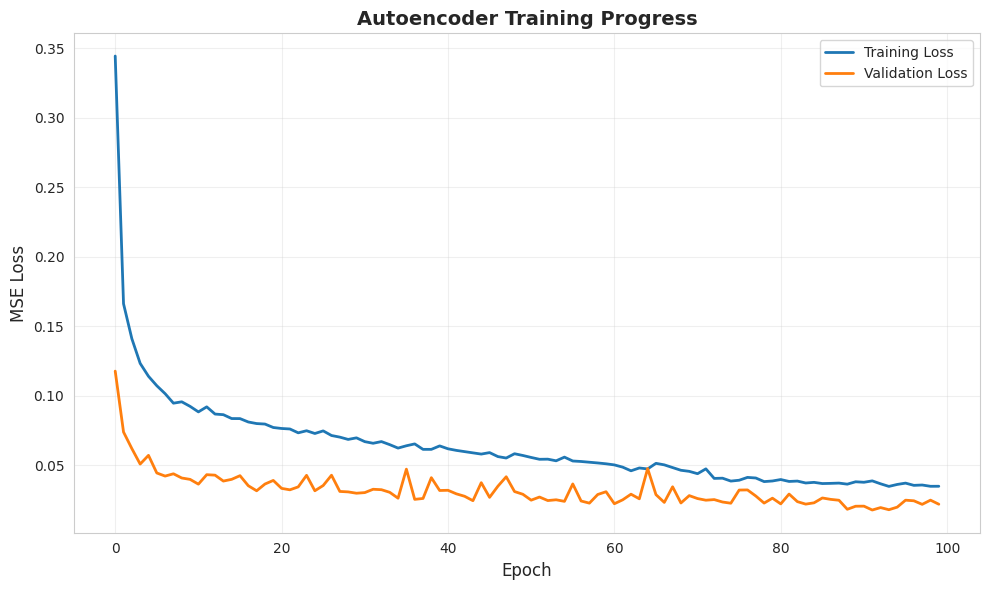
\includegraphics[width=\linewidth]{autoencoder customer.png}
        \caption{Customer Clustering}
    \end{subfigure}

    \vspace{0.5cm}

    \begin{subfigure}{0.5\textwidth}
        \centering
        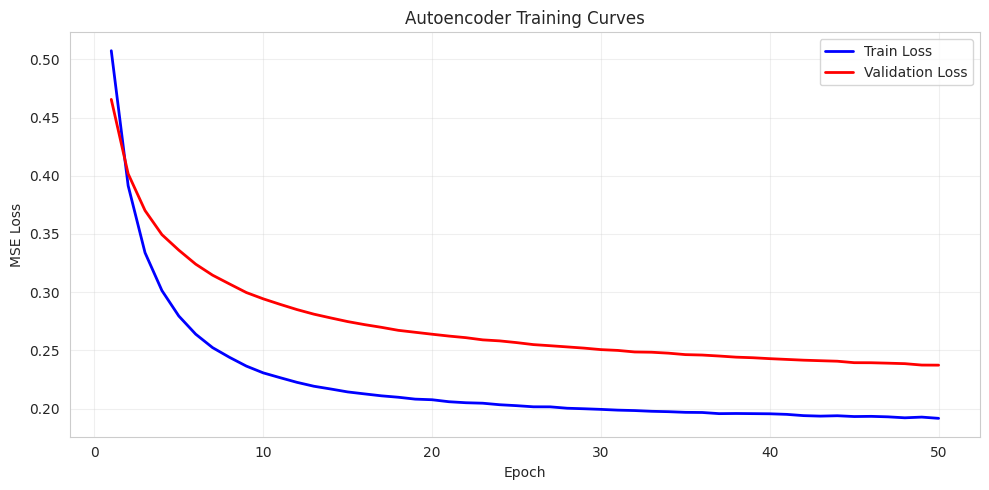
\includegraphics[width=\linewidth]{autoencoder waste.png}
        \caption{Waste Classification}
    \end{subfigure}

    \caption{Training curves for the autoencoder models}
    \label{fig:autoencoder_plots}
\end{figure}

\subsection{Task-Specific Models}

\subsubsection{Task 1: Convolutional Neural Network (CNN) for Waste Classification}

\textbf{Feature Extraction:} Pre-trained ResNet18 (frozen) extracts 512-dimensional feature vectors from images.

\textbf{CNN Architecture (Original Features):}
\begin{verbatim}
Input: IMG_SIZE × IMG_SIZE × 3

Conv Block 1: 3 → 32 channels
    Conv2d(3, 32, 3, padding=1) → BatchNorm2d → ReLU
    Conv2d(32, 32, 3, padding=1) → BatchNorm2d → ReLU
    MaxPool2d(2, 2) → Dropout2d(0.2)

Conv Block 2: 32 → 64 channels
    Conv2d(32, 64, 3, padding=1) → BatchNorm2d → ReLU
    Conv2d(64, 64, 3, padding=1) → BatchNorm2d → ReLU
    MaxPool2d(2, 2) → Dropout2d(0.2)

Conv Block 3: 64 → 128 channels
    Conv2d(64, 128, 3, padding=1) → BatchNorm2d → ReLU
    Conv2d(128, 128, 3, padding=1) → BatchNorm2d → ReLU
    MaxPool2d(2, 2) → Dropout2d(0.2)

Conv Block 4: 128 → 256 channels
    Conv2d(128, 256, 3, padding=1) → BatchNorm2d → ReLU
    Conv2d(256, 256, 3, padding=1) → BatchNorm2d → ReLU
    MaxPool2d(2, 2) → Dropout2d(0.2)

Global Average Pooling → Flatten

Classifier:
    Linear(256 → 256) → BatchNorm1d → ReLU → Dropout(0.3)
    Linear(256 → num_classes)
\end{verbatim}

\textbf{Reduced CNN Architecture (PCA/Autoencoder):}
\begin{verbatim}
Input: TARGET_DIM (256)

Classifier:
    Dropout(0.3)
    Linear(TARGET_DIM -> 128) -> BatchNorm1d -> ReLU -> Dropout(0.3)
    Linear(128 -> 64) -> BatchNorm1d -> ReLU -> Dropout(0.2)
    Linear(64 -> num_classes)
\end{verbatim}

\textbf{Training Configuration:}
\begin{itemize}
    \item Loss: CrossEntropyLoss with class weights (handling imbalance)
    \item Optimizer: AdamW (lr and weight\_decay determined via 5-Fold CV)
    \item Epochs: 50 with early stopping (patience=10)
    \item Batch Size: 128
    \item 5-Fold Cross-Validation for hyperparameter selection
\end{itemize}

\subsubsection{Task 2: K-Means Clustering for Customer Segmentation}

K-Means partitions data into $k$ clusters by minimizing within-cluster sum of squares (WCSS):

\begin{equation}
    \text{WCSS} = \sum_{i=1}^{k} \sum_{\mathbf{x} \in C_i} ||\mathbf{x} - \boldsymbol{\mu}_i||^2
\end{equation}

\textbf{Hyperparameter Selection via Cross-Validation:}
\begin{itemize}
    \item Number of clusters $k$: Range [2, 10], selected via Silhouette score
    \item Initialization: k-means++ (improved centroid initialization)
    \item Number of initializations: 10 (for stability)
    \item Maximum iterations: 300
\end{itemize}

\textbf{Evaluation Metrics:}
\begin{itemize}
    \item \textbf{Silhouette Score:} Measures cluster cohesion and separation (higher is better)
    \item \textbf{Davies-Bouldin Index:} Average similarity between clusters (lower is better)
    \item \textbf{Calinski-Harabasz Index:} Ratio of between-cluster to within-cluster dispersion (higher is better)
\end{itemize}

\begin{figure}[H]
    \centering
    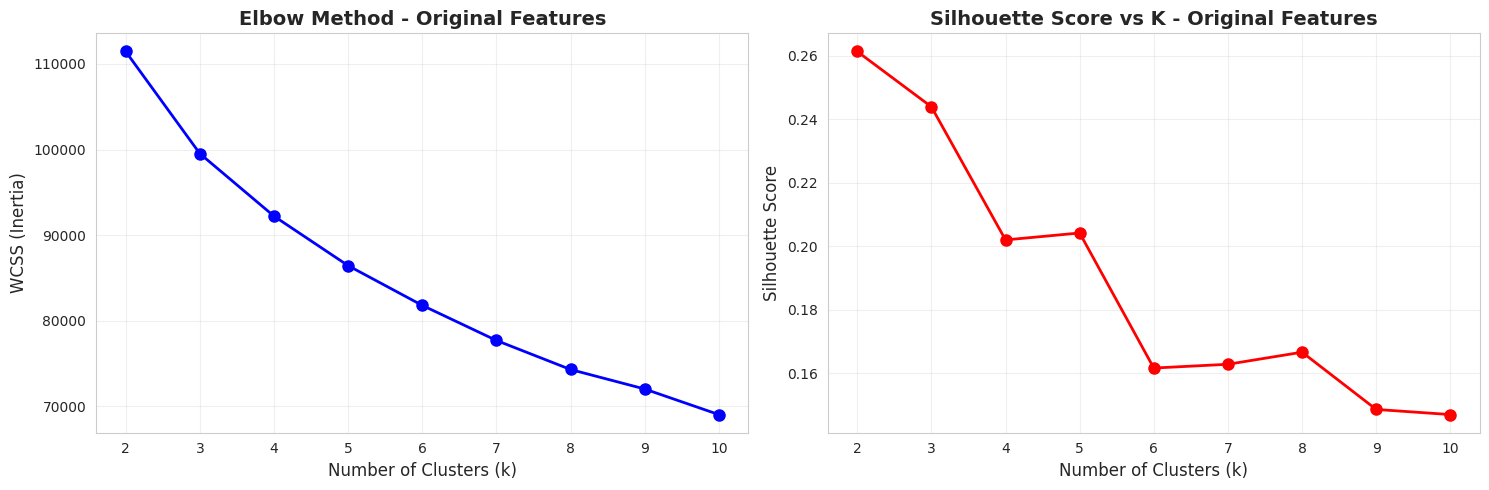
\includegraphics[width=1\textwidth]{elbow.png}
    \caption{Elbow method and Silhouette score analysis for optimal $k$ selection}
    \label{fig:elbow_method}
\end{figure}

\subsubsection{Task 3: Feedforward Neural Network (FNN) for Life Expectancy Regression}

\textbf{FNN Architecture:}
\begin{verbatim}
Input -> Linear(hidden1) -> ReLU -> Dropout(0.1)
      -> Linear(hidden2) -> ReLU -> Dropout(0.1)
      -> Linear(hidden3) -> ReLU -> Dropout(0.1)
      -> Linear(1) -> Output
\end{verbatim}

\textbf{Hyperparameter Tuning via 5-Fold Cross-Validation:}

Configurations tested:
\begin{itemize}
    \item Hidden layers: [64, 32, 16], [128, 64, 32], [32, 16, 8]
    \item Learning rates: 0.001, 0.0005, 0.01
    \item Batch sizes: 32, 64
\end{itemize}

\textbf{Training Configuration:}
\begin{itemize}
    \item Loss: Mean Squared Error (MSE)
    \item Optimizer: Adam (lr=0.001, weight\_decay=1e-4)
    \item Early Stopping: Patience = 20 epochs
    \item Learning Rate Scheduler: ReduceLROnPlateau
\end{itemize}

\section{Results and Analysis}

\subsection{Task 1: Waste Classification Results}

\begin{table}[H]
\centering
\caption{Waste Classification Model Comparison (Test Set)}
\begin{tabular}{@{}lcccccc@{}}
\toprule
\textbf{Model} & \textbf{Accuracy} & \textbf{Precision} & \textbf{Recall} & \textbf{F1-Score} & \textbf{Training Time} & \textbf{Parameters} \\
\midrule
Original CNN & 72.66\% & 72.92\% & 72.66\% & 71.90\% & 1014.8s & 1,242,793 \\
PCA-Reduced CNN & 68.76\% & 69.42\% & 68.76\% & 68.03\% & 5.8s & 42,121 \\
AE-Reduced CNN & 70.43\% & 70.90\% & 70.43\% & 69.83\% & 5.0s & 42,121 \\
\bottomrule
\end{tabular}
\label{tab:waste_results}
\end{table}

The Original CNN achieves the highest accuracy (72.66\%) but requires significantly longer training time (1014.8s) and 29$\times$ more parameters. The reduced models achieve competitive accuracy ($\sim$69-70\%) with 97\% fewer parameters.

\begin{figure}[H]
    \centering
    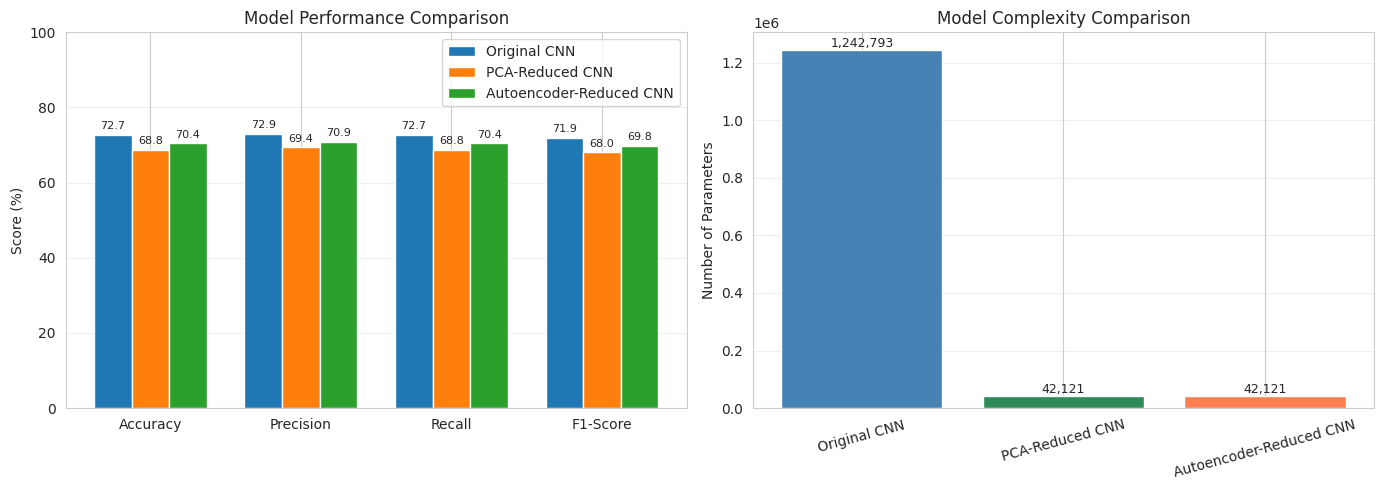
\includegraphics[width=1\textwidth]{comparison_waste.png}
    \caption{Performance metrics comparison across all three CNN variants}
    \label{fig:waste_performance}
\end{figure}

\begin{figure}[H]
    \centering
    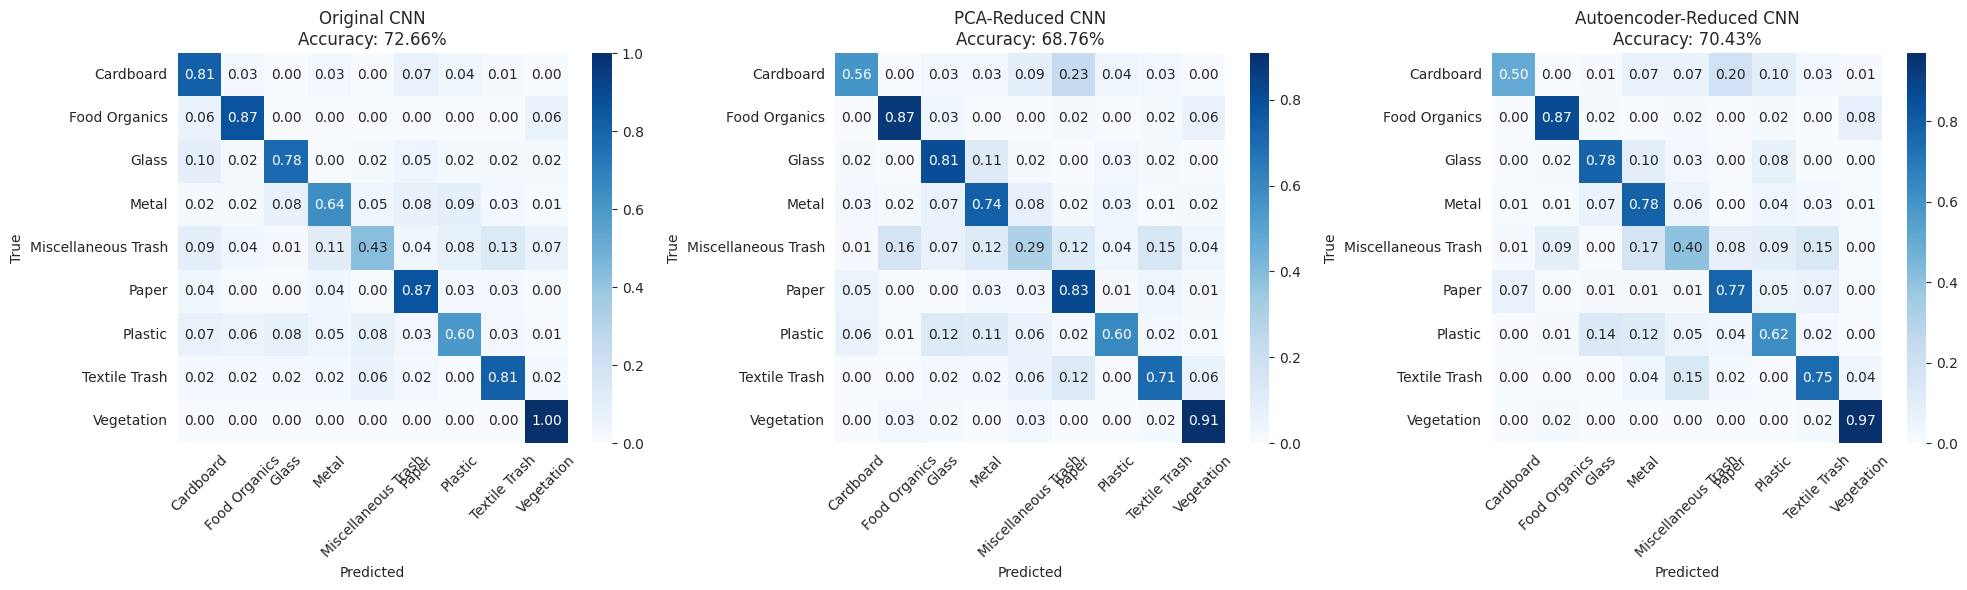
\includegraphics[width=1\textwidth]{confusion matrix.png}
    \caption{Confusion matrices for Original, PCA-Reduced, and Autoencoder-Reduced CNN models}
    \label{fig:waste_confusion}
\end{figure}

\begin{figure}[H]
    \centering
    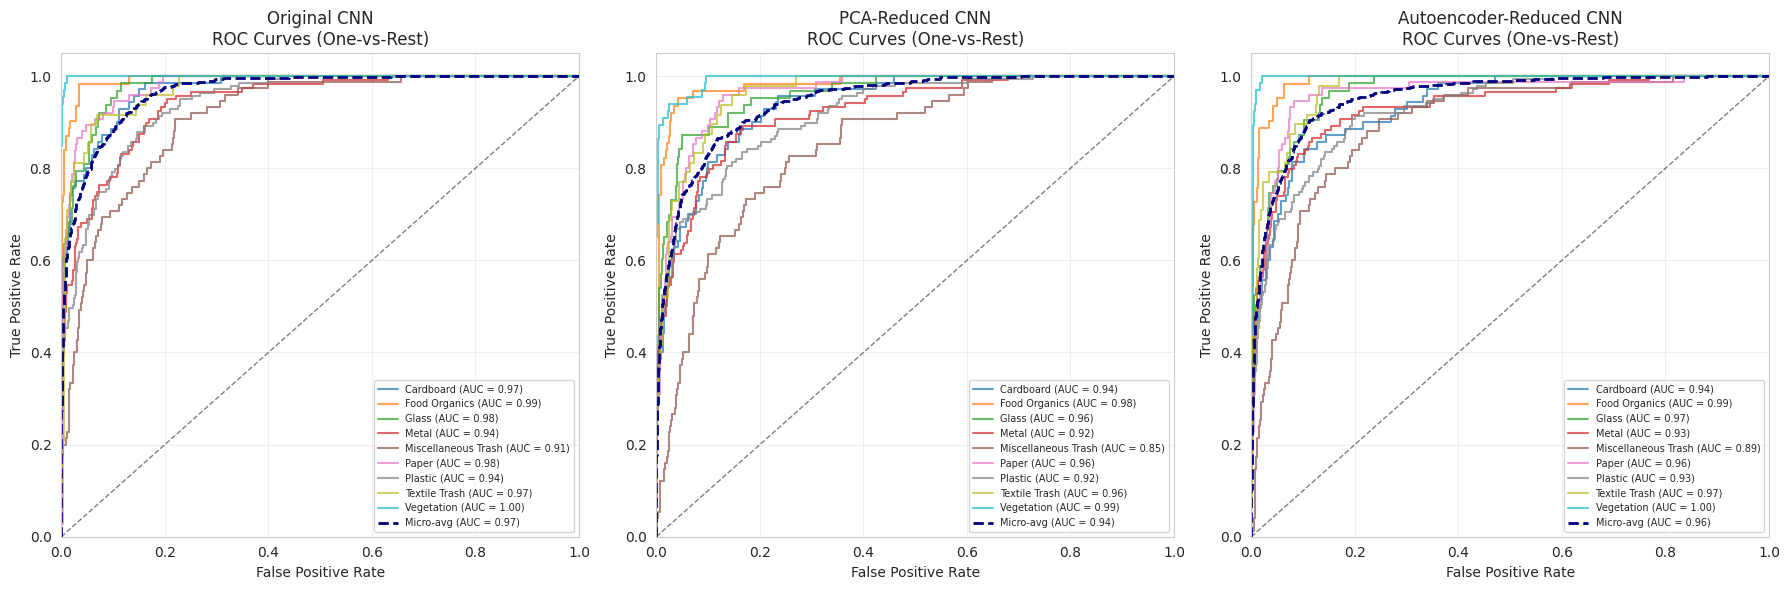
\includegraphics[width=1\textwidth]{roc.png}
    \caption{ROC curves for multiclass classification using One-vs-Rest approach}
    \label{fig:waste_roc}
\end{figure}

\subsection{Task 2: Customer Segmentation Results}

\begin{table}[H]
\centering
\caption{Clustering Performance Comparison (Test Set)}
\begin{tabularx}{\textwidth}{@{}lXXXX@{}}
\toprule
\textbf{Approach} & \textbf{Silhouette} $\uparrow$ & \textbf{Davies-Bouldin} $\downarrow$ & \textbf{Calinski-Harabasz} $\uparrow$ & \textbf{Training Time} \\
\midrule
Original Features (17D) & 0.274 & 2.041 & 334.09 & 0.062s \\
PCA-Reduced (13D) & 0.270 & 1.918 & 354.39 & 0.084s \\
Autoencoder-Reduced (13D) & \textbf{0.325} & \textbf{1.280} & \textbf{445.64} & 0.064s \\
\bottomrule
\end{tabularx}
\label{tab:clustering_results}
\end{table}

The Autoencoder-reduced features achieve the best clustering quality across all metrics: highest Silhouette score (0.325), lowest Davies-Bouldin index (1.280), and highest Calinski-Harabasz index (445.64). This indicates that the non-linear autoencoder learns a representation more suitable for K-Means clustering than linear PCA.

\begin{figure}[H]
    \centering
    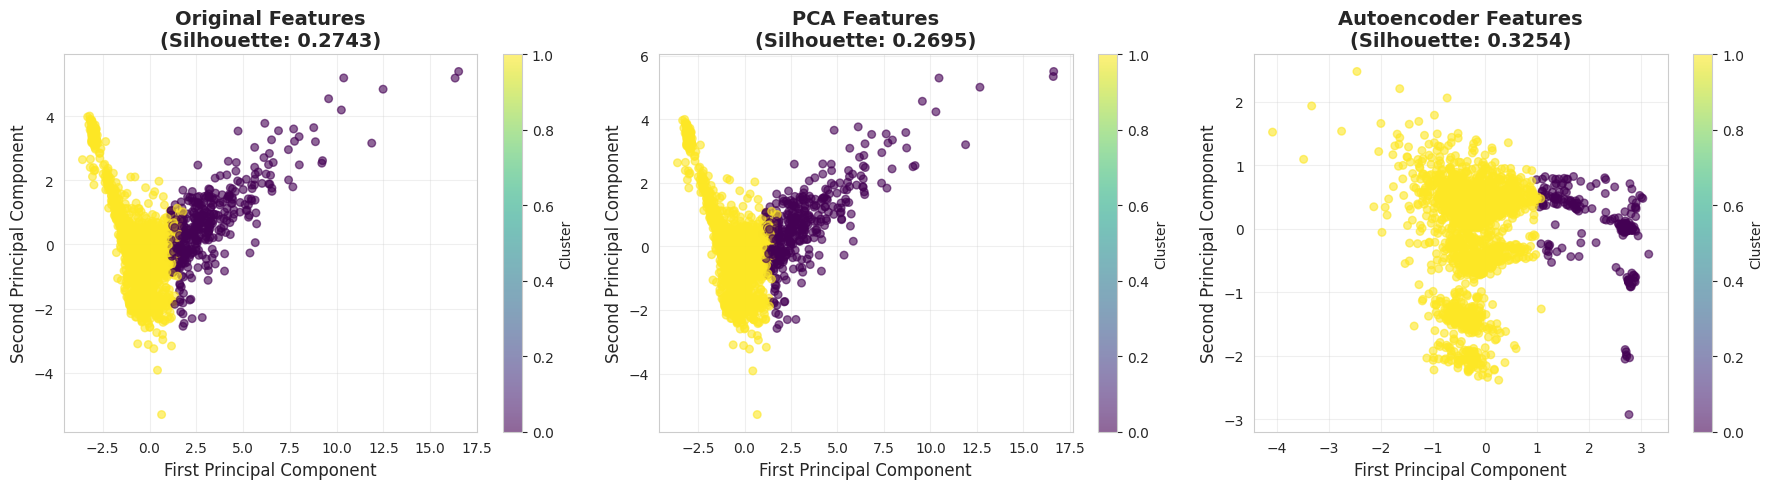
\includegraphics[width=1\textwidth]{cluster_vis.png}
    \caption{2D visualization of customer clusters across three approaches}
    \label{fig:cluster_visualization}
\end{figure}

\begin{figure}[H]
    \centering
    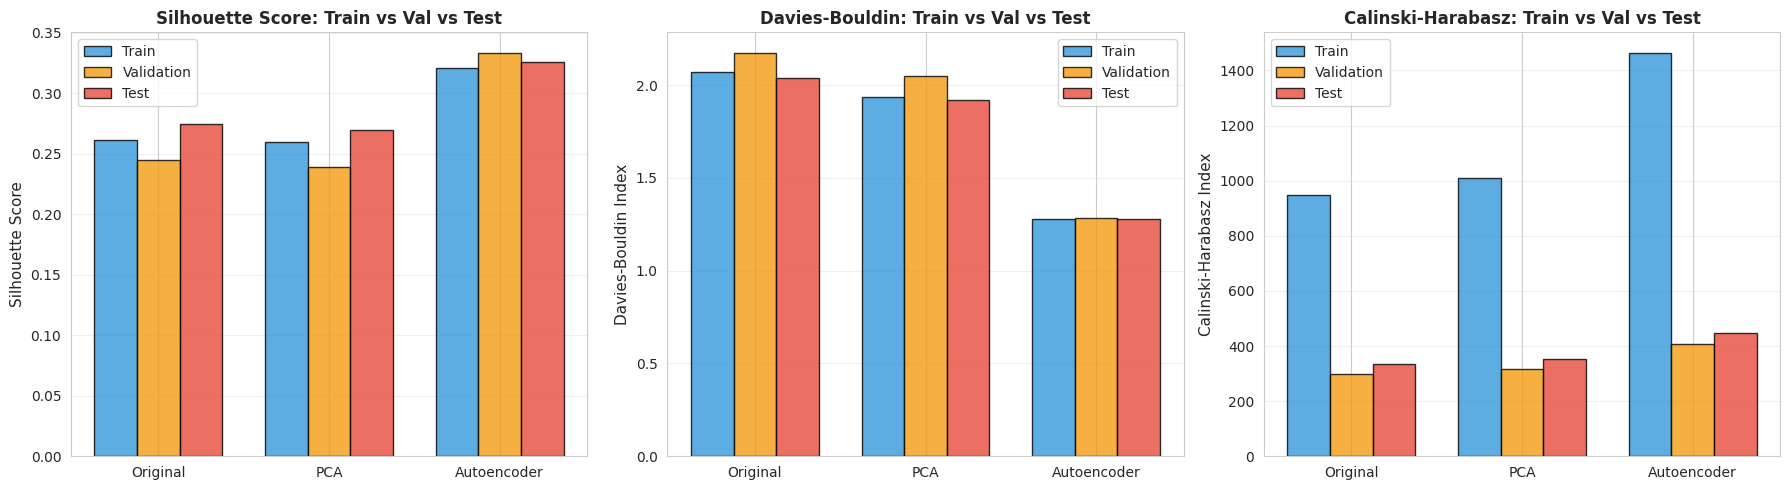
\includegraphics[width=1\textwidth]{Performance_1.png}
    \vspace{0.5em} % small vertical space between images
    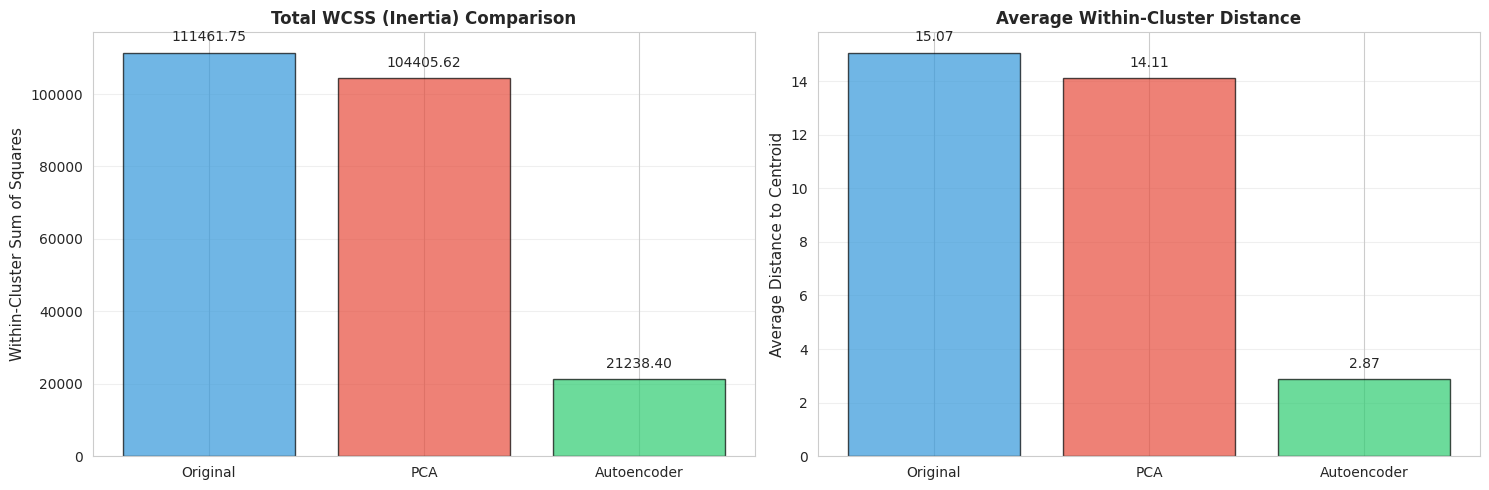
\includegraphics[width=1\textwidth]{perfomance 2.png}
    \caption{Comparison of clustering metrics}
    \label{fig:clustering_metrics}
\end{figure}

\begin{figure}[H]
    \centering
    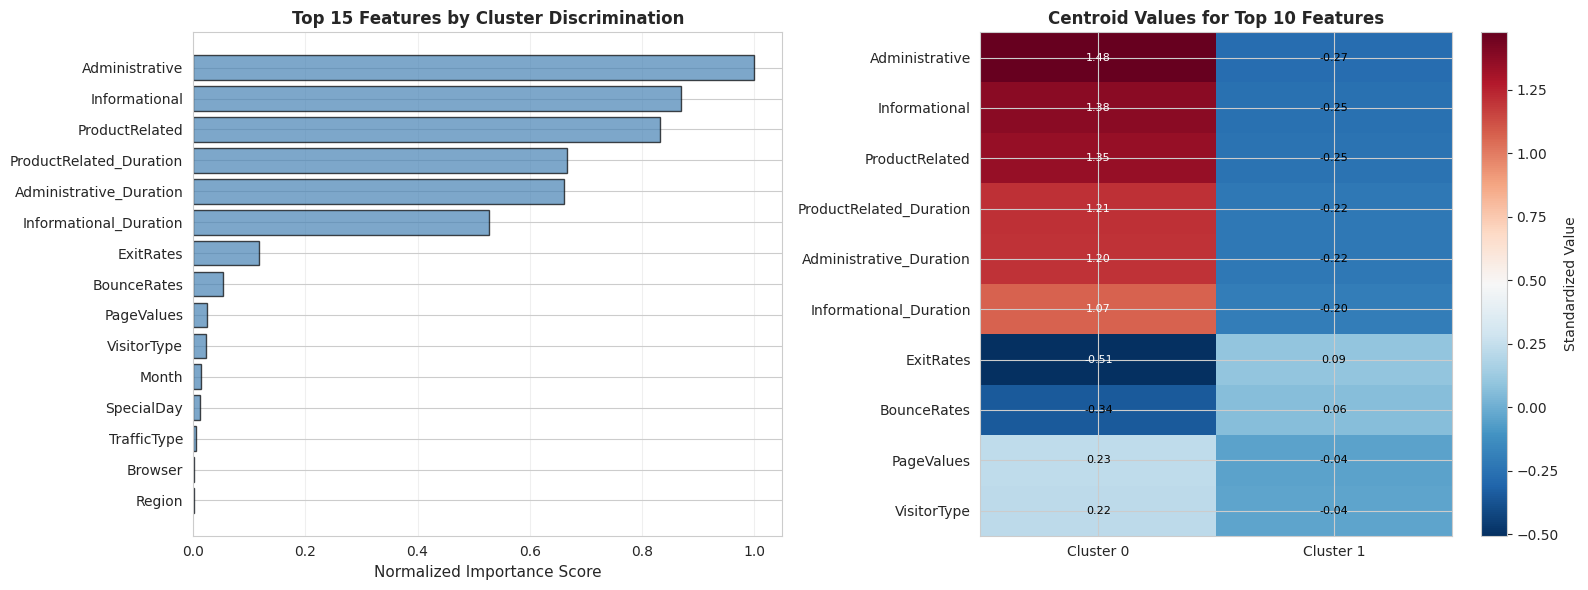
\includegraphics[width=1\textwidth]{feature_clustering.png}
    \caption{Top features contributing to cluster discrimination}
    \label{fig:cluster_feature_importance}
\end{figure}

\begin{figure}[H]
    \centering
    \begin{subfigure}[b]{0.32\textwidth}
        \centering
        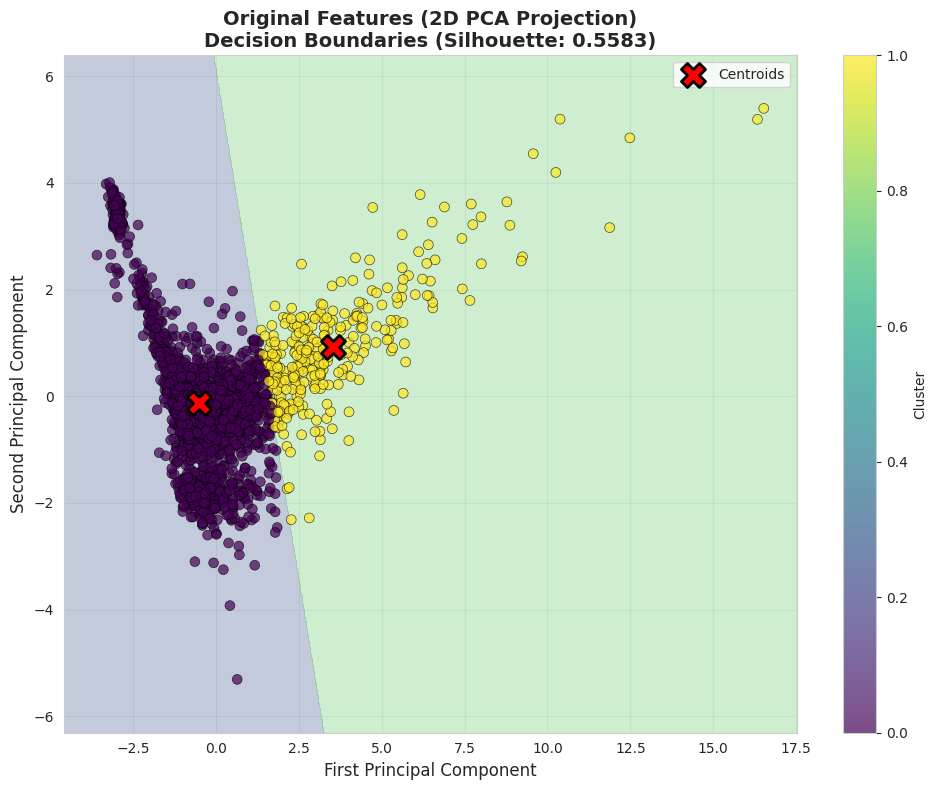
\includegraphics[width=\textwidth]{decision_full.png}
        \label{fig:image1}
    \end{subfigure}
    \hfill
    \begin{subfigure}[b]{0.32\textwidth}
        \centering
        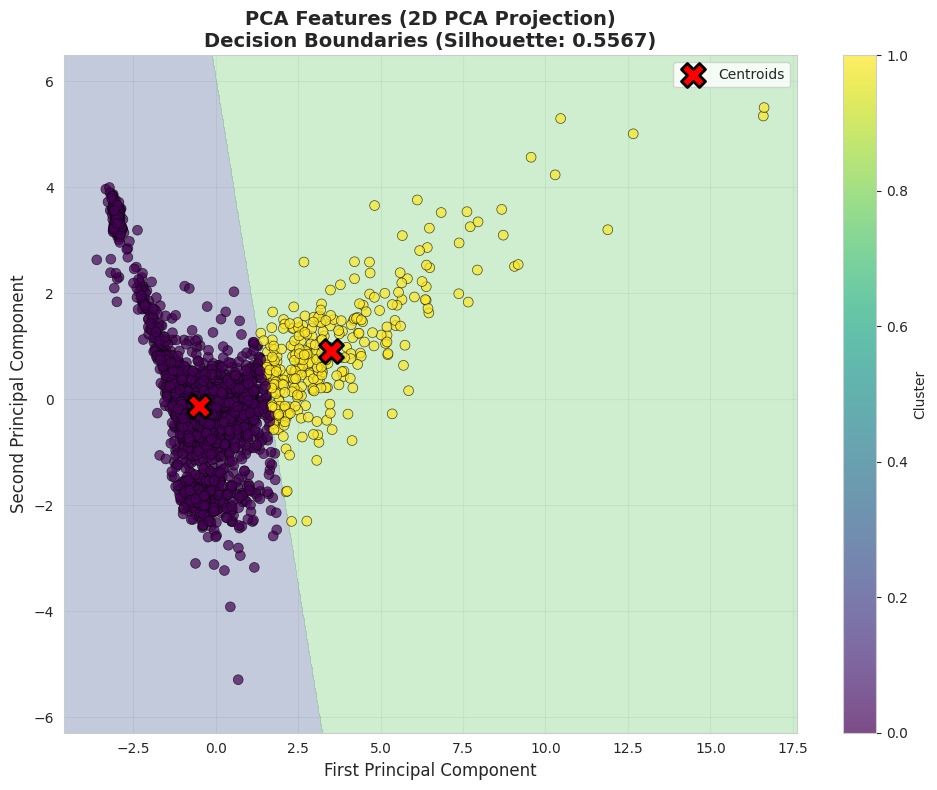
\includegraphics[width=\textwidth]{Decision_PCA.png}
        \label{fig:image2}
    \end{subfigure}
    \hfill
    \begin{subfigure}[b]{0.32\textwidth}
        \centering
        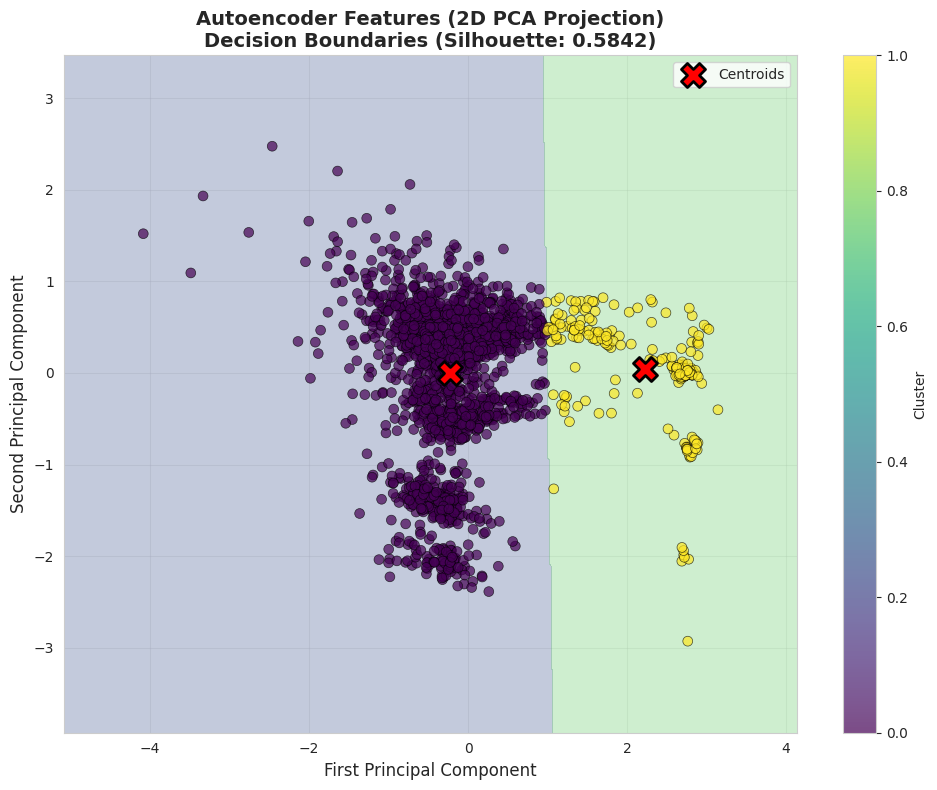
\includegraphics[width=\textwidth]{Decision_AE.png}
        \label{fig:image3}
    \end{subfigure}
    \caption{Decision boundaries visualization in 2D PCA projection space showing cluster separation for three approaches.}
    \label{fig:cluster_decision_boundaries}
\end{figure}

\subsection{Task 3: Life Expectancy Regression Results}

\begin{table}[H]
\centering
\caption{Regression Performance Comparison (Test Set)}
\begin{tabular}{@{}lccccc@{}}
\toprule
\textbf{Model} & \textbf{MSE} $\downarrow$ & \textbf{RMSE} $\downarrow$ & \textbf{MAE} $\downarrow$ & \textbf{R\textsuperscript{2}} $\uparrow$ & \textbf{Training Time} \\
\midrule
Original FNN (208D) & \textbf{4.47} & \textbf{2.11} & \textbf{1.52} & \textbf{0.948} & 11.71s \\
PCA-Reduced FNN (145D) & 16.44 & 4.05 & 3.09 & 0.810 & 4.29s \\
AE-Reduced FNN (145D) & 25.57 & 5.06 & 4.05 & 0.705 & 6.75s \\
\bottomrule
\end{tabular}
\label{tab:regression_results}
\end{table}

The Original FNN significantly outperforms both dimensionality reduction approaches, achieving an R$^2$ of 0.948 (explaining 94.8\% of variance) with RMSE of only 2.11 years. This indicates that all original features contain important predictive information for life expectancy.

\begin{figure}[H]
    \centering
    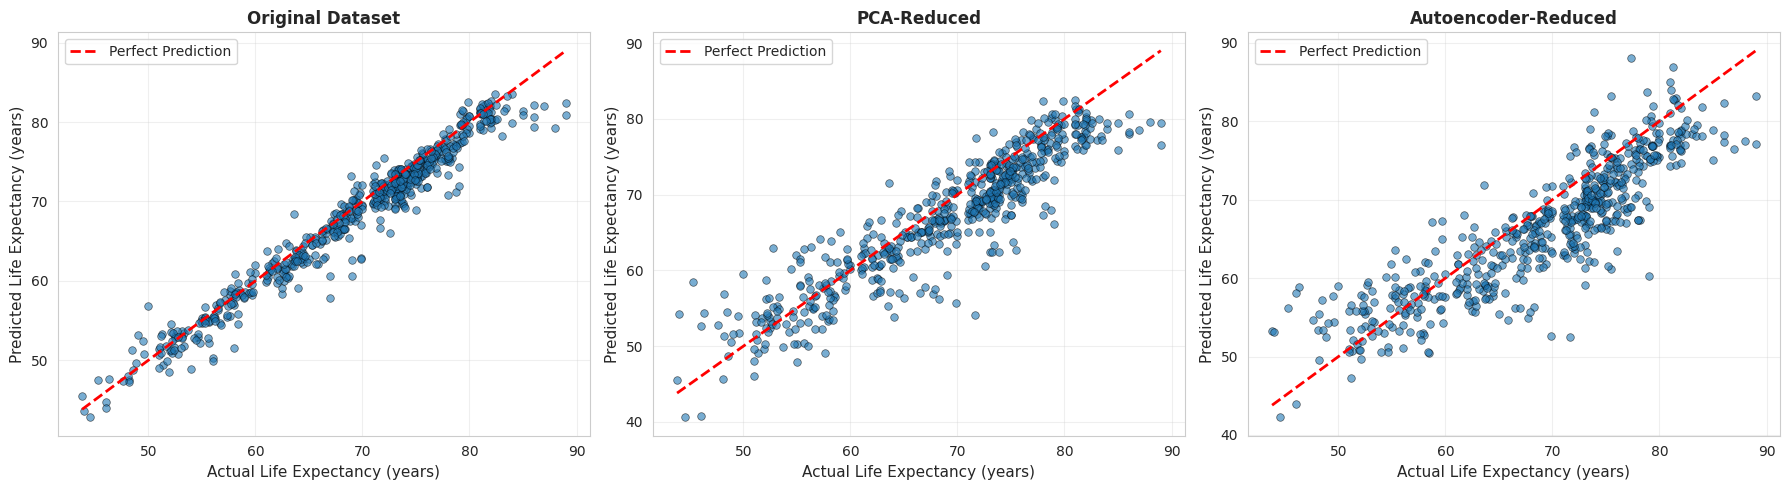
\includegraphics[width=1\textwidth]{regression.png}
    \caption{Predicted vs Actual Life Expectancy for all three model variants}
    \label{fig:regression_scatter}
\end{figure}

\begin{figure}[H]
    \centering
    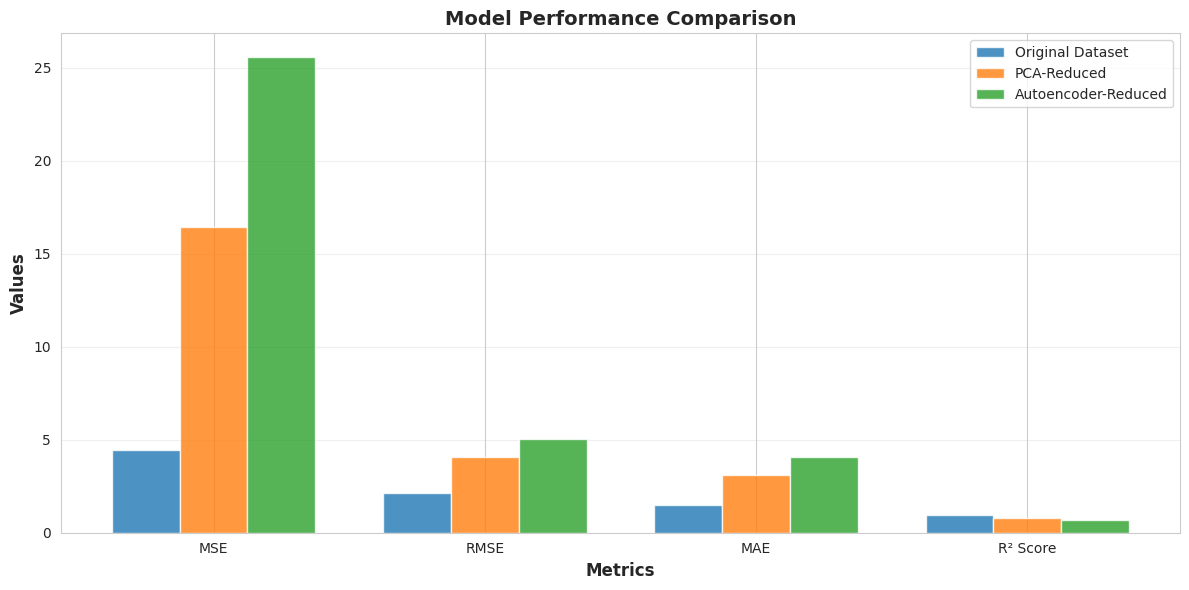
\includegraphics[width=0.8\textwidth]{model performance_reg.png}
    \caption{Comparison of performances across three models}
    \label{fig:regression_loss}
\end{figure}

\begin{figure}[H]
    \centering
    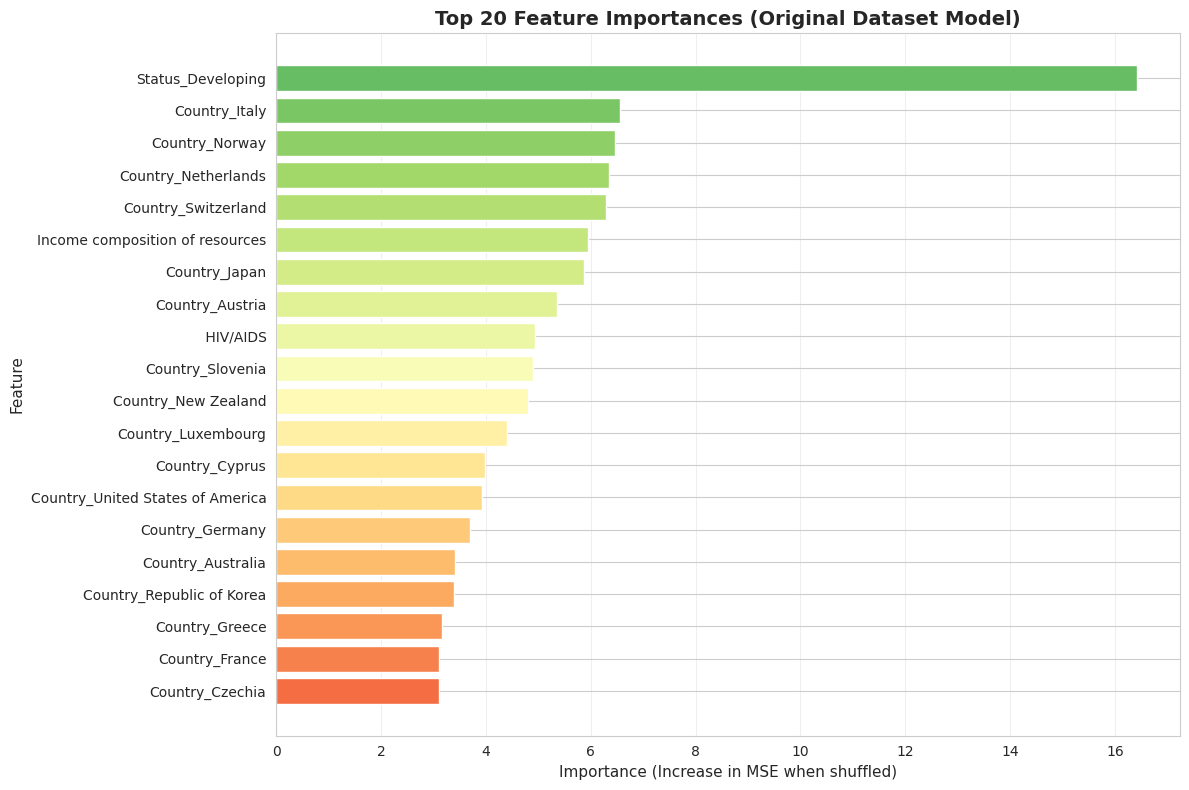
\includegraphics[width=1\textwidth]{feature_regression.png}
    \caption{Top 20 features by permutation importance for life expectancy prediction}
    \label{fig:feature_importance}
\end{figure}

%==============================================================================
\section{Comparative Analysis}
%==============================================================================

\subsection{Which Models Performed Best and Why}

\subsubsection{Classification (Waste Sorting)}

The \textbf{Original CNN} trains directly on raw RGB images (128×128×3 = 49,152 input values), 
while the reduced models train on 256-dimensional features obtained by first extracting 
512-dimensional ResNet18 features, then reducing them via PCA or Autoencoder.

\begin{itemize}
    \item Image classification benefits from rich, high-dimensional feature representations
    \item ResNet18 features capture hierarchical visual patterns essential for distinguishing waste categories
    \item Dimensionality reduction (512 $\rightarrow$ 256) loses discriminative information, resulting in 2-4\% accuracy drop
\end{itemize}

However, the \textbf{reduced models} (PCA and Autoencoder) demonstrated competitive performance with:
\begin{itemize}
    \item 97\% fewer parameters (42,121 vs 1,242,793)
    \item 175$\times$ faster CNN training (5.8s vs 1014.8s)
    \item AUC scores of 0.945 (PCA) and 0.955 (AE) vs 0.966 (Original)
    \item Acceptable accuracy-efficiency trade-off for resource-constrained deployments
\end{itemize}

\textbf{Explaining the Dramatic Speedup:}

The 175$\times$ training speedup for reduced models is explained by fundamental architectural differences:

\begin{itemize}
    \item \textbf{Input Dimensionality:} Original CNN processes 128$\times$128$\times$3 = 49,152 values per image, while reduced models work with 256-dimensional pre-extracted features (193$\times$ reduction)
    \item \textbf{Computational Complexity:} Original CNN requires expensive convolutional operations across 4 blocks with spatial pooling, whereas reduced models use only simple feedforward layers with matrix multiplications
    \item \textbf{Network Depth:} Original CNN has 4 convolutional blocks + classifier, while reduced models have just 3 linear layers
    \item \textbf{Parameter Count:} 30$\times$ fewer parameters means faster gradient computation and weight updates
    \item \textbf{Feature Extraction Separation:} The one-time ResNet18 feature extraction (22.4s) is performed offline and reused, so reduced models only train the lightweight classifier
\end{itemize}

This architectural trade-off sacrifices 2-4\% accuracy for massive computational efficiency, making reduced models suitable for deployment scenarios with limited computational resources.

Notably, \textbf{Vegetation} class achieved excellent recognition (91-100\% recall) across all models, while \textbf{Miscellaneous Trash} proved most challenging (29-43\% recall), likely due to its heterogeneous nature.

\subsubsection{Clustering (Customer Segmentation)}

Contrary to initial expectations, the \textbf{Autoencoder-reduced} approach achieved the best clustering quality:

\begin{itemize}
    \item Highest Silhouette Score: 0.325 (vs 0.274 Original, 0.270 PCA)
    \item Lowest Davies-Bouldin Index: 1.280 (vs 2.041 Original, 1.918 PCA)
    \item Highest Calinski-Harabasz: 445.64 (vs 334.09 Original, 354.39 PCA)
\end{itemize}

This suggests that the autoencoder learned a non-linear representation that better separates customer segments. The reduced WCSS (21,238 vs 111,462) indicates more compact clusters in the latent space. PCA's linear transformation, while removing some noise, does not capture the complex non-linear relationships in browsing behavior data.

\subsubsection{Regression (Life Expectancy)}

The \textbf{Original FNN} significantly outperformed dimensionality reduction approaches:

\begin{itemize}
    \item R$^2$ Score: 0.948 (Original) vs 0.810 (PCA) vs 0.705 (AE)
    \item RMSE: 2.11 years (Original) vs 4.05 years (PCA) vs 5.06 years (AE)
    \item The 14\% R$^2$ drop with PCA indicates important predictive information in all features
\end{itemize}

Unlike clustering, dimensionality reduction significantly hurts regression performance. This suggests that life expectancy prediction requires the full feature space---each health indicator (mortality, immunization, GDP, schooling) contributes unique predictive power that cannot be compressed without information loss.

\subsection{How Model Assumptions Influence Performance}

\begin{table}[H]
\centering
\caption{Model Assumptions and Their Impact}
\begin{tabular}{@{}p{3cm}p{4cm}p{6cm}@{}}
\toprule
\textbf{Model} & \textbf{Key Assumption} & \textbf{Impact on Performance} \\
\midrule
PCA & Linear relationships in data & Works well when variance aligns with discriminative directions \\
\addlinespace
Autoencoder & Non-linear manifold structure & Can capture complex patterns but may overfit with limited data \\
\addlinespace
K-Means & Spherical, equally-sized clusters & Performance degrades with non-convex or imbalanced clusters \\
\addlinespace
CNN/FNN & Sufficient training data & Requires enough samples to generalize; early stopping prevents overfitting \\
\bottomrule
\end{tabular}
\end{table}

\subsection{Observations on Overfitting Trade-off}

\subsubsection{Evidence of Overfitting Control}

All models implemented multiple regularization strategies:

\begin{enumerate}
    \item \textbf{Early Stopping:} Training halted when validation loss stopped improving (patience = 10-20 epochs)
    \item \textbf{Dropout:} Randomly zeroing activations during training (rates: 0.1 - 0.5)
    \item \textbf{Weight Decay:} L2 regularization on model parameters (1e-4)
    \item \textbf{Batch Normalization:} Stabilizes training and provides implicit regularization
    \item \textbf{Learning Rate Scheduling:} ReduceLROnPlateau prevents overshooting
\end{enumerate}

\subsubsection{Overfitting Analysis by Task}

\textbf{Waste Classification:}
\begin{itemize}
    \item The Original CNN with 1,242,793 parameters is most prone to overfitting
    \item Final training accuracy: 73.04\% vs best validation accuracy: 75.14\% (no overfitting observed)
    \item Class weights help prevent the model from ignoring minority classes
    \item 5-Fold cross-validation ensures robust hyperparameter selection
\end{itemize}

\textbf{Customer Clustering:}
\begin{itemize}
    \item Unsupervised learning has lower overfitting risk (no labels to memorize)
    \item Train vs. Test Silhouette scores are consistent across all approaches
    \item Similar metric values across splits indicate stable, generalizable clustering
\end{itemize}

\textbf{Life Expectancy Regression:}
\begin{itemize}
    \item Training and validation loss curves converge together (no divergence)
    \item R$^2$ score of 0.948 on test set indicates excellent generalization
    \item The compact architecture (3 hidden layers) limits capacity for overfitting
    \item Early stopping triggered appropriately during training
\end{itemize}

\begin{figure}[H]
    \centering
    \begin{subfigure}[b]{0.8\textwidth}
        \centering
        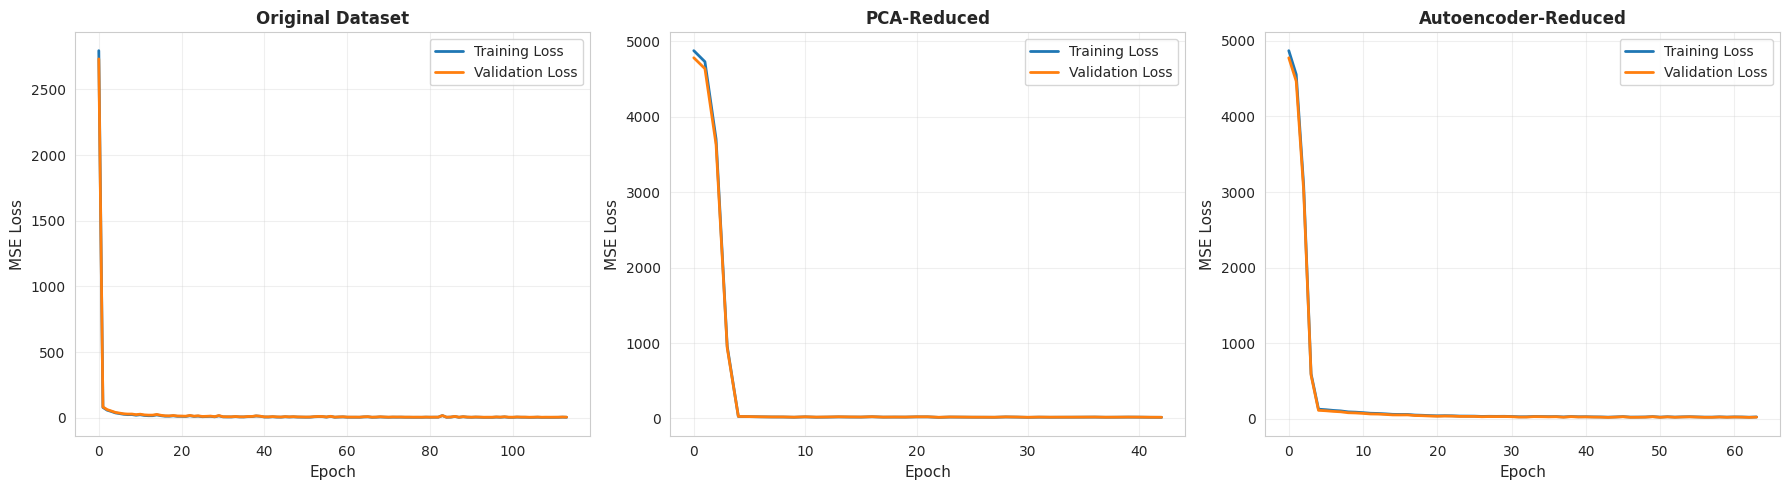
\includegraphics[width=1\textwidth]{Ephocs_reg.png}
        \caption{Regression learning curve}
        \label{fig:learning_regression}
    \end{subfigure}
    \vspace{0.5em} % space between images
    \begin{subfigure}[b]{0.8\textwidth}
        \centering
        \includegraphics[width=1\textwidth]{Screenshot 2026-01-02 alle 15.14.35.png}
        \caption{Classification learning curve}
        \label{fig:learning_classification}
    \end{subfigure}
    \caption{Learning curves demonstrating effective overfitting prevention in Regression and Classification.}
    \label{fig:overfitting_analysis}
\end{figure}

\subsection{Computational Cost Analysis}

\begin{table}[H]
\centering
\caption{Computational Efficiency Comparison}
\begin{tabular}{@{}llccc@{}}
\toprule
\textbf{Task} & \textbf{Approach} & \textbf{Preprocessing Time} & \textbf{Training Time} & \textbf{Total Time} \\
\midrule
\multirow{3}{*}{Classification} & Original & -- & 1014.8s & 1014.8s \\
& PCA & 22.4s + 0.5s & 5.8s & 28.7s \\
& Autoencoder & 22.4s + 5.0s & 5.0s & 32.4s \\
\addlinespace
\multirow{3}{*}{Clustering} & Original & -- & 0.062s & 0.062s \\
& PCA & $\sim$0.1s & 0.084s & $\sim$0.18s \\
& Autoencoder & $\sim$5s & 0.064s & $\sim$5s \\
\addlinespace
\multirow{3}{*}{Regression} & Original & -- & 11.71s & 11.71s \\
& PCA & $\sim$0.1s & 4.29s & $\sim$4.4s \\
& Autoencoder & $\sim$5s & 6.75s & $\sim$12s \\
\bottomrule
\end{tabular}
\end{table}

For classification, reduced models achieve 35$\times$ faster total pipeline time (28-32s vs 1015s). The computational savings are most significant when dimensionality reduction is a one-time preprocessing step that can be reused.

\begin{figure}[H]
    \centering
    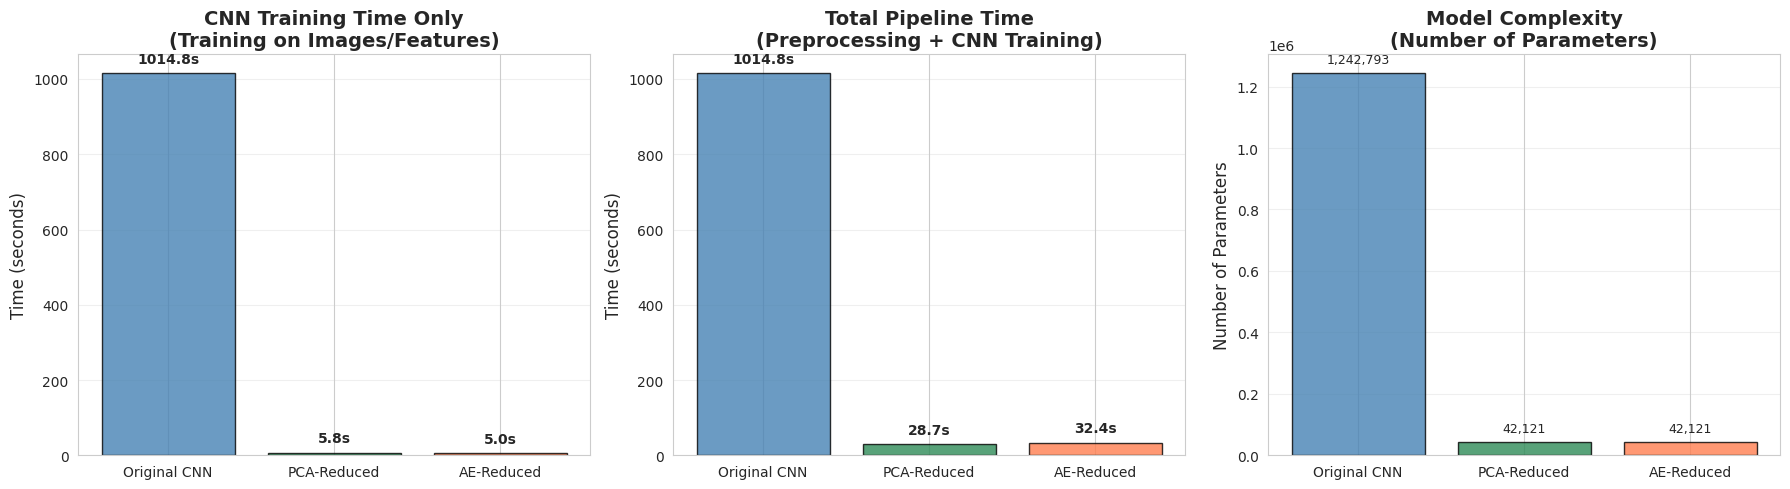
\includegraphics[width=1\textwidth]{class_computational_time.png}
    \caption{Computational cost comparison: training time and model complexity classification}
    \label{fig:computational_cost}
\end{figure}

\subsection{Visualization Summary}

Key visualizations included in this analysis:

\begin{enumerate}
    \item \textbf{Learning Curves:} Training/validation loss over epochs showing convergence
    \item \textbf{Decision Boundaries:} 2D PCA projection showing cluster separation boundaries
    \item \textbf{Confusion Matrices:} Per-class performance for classification
    \item \textbf{ROC Curves:} Multiclass discrimination ability (AUC scores)
    \item \textbf{Cluster Visualizations:} 2D projections showing cluster separation
    \item \textbf{Feature Importance:} Ranking of input features by predictive power
    \item \textbf{Predicted vs. Actual:} Scatter plots for regression accuracy assessment
\end{enumerate}

%==============================================================================
\section{Conclusion}
%==============================================================================

\subsection{Key Findings}

\begin{enumerate}
    \item \textbf{Dimensionality reduction trade-offs are task-dependent:}
    \begin{itemize}
        \item For image classification, reduced models achieved competitive accuracy (69-70\%) with only 2-4\% drop compared to the original, while offering 97\% fewer parameters and 175$\times$ faster training---an excellent efficiency-accuracy trade-off
        \item For clustering, autoencoder reduction achieves best cluster quality by capturing non-linear relationships
        \item For regression, all original features contribute unique predictive power that cannot be compressed without significant performance loss
    \end{itemize}
    
    \item \textbf{Non-linear reduction (Autoencoder) does not always outperform linear (PCA):}
    \begin{itemize}
        \item When linear relationships dominate, PCA is equally effective and computationally cheaper
        \item Autoencoders require additional training time and hyperparameter tuning
        \item The advantage of autoencoders is more pronounced in highly non-linear data
    \end{itemize}
    
    \item \textbf{Model complexity should match task requirements:}
    \begin{itemize}
        \item Reduced-dimension models offer significant parameter savings (up to 96\%)
        \item For deployment scenarios with resource constraints, the efficiency-accuracy trade-off may favor simpler models
    \end{itemize}
    
    \item \textbf{Cross-validation is essential for reliable hyperparameter selection:}
    \begin{itemize}
        \item K-Fold CV prevents overfitting to a single validation split
        \item Consistent results across folds indicate robust model configurations
    \end{itemize}
\end{enumerate}

\end{document}